\section{问题描述}
\newcommand{\myP}{40kW}
\newcommand{\myn}{100r/min}
\newcommand{\myda}{688mm}
\newcommand{\mybetaa}{$12^\circ 50'$}
\newcommand{\mydb}{170mm}
\newcommand{\mybetab}{$10^\circ 29'$}
设计二级斜齿圆柱齿轮减速器,已知参数如表\ref{tab:para}所示。
\begin{table}[H]
\centering
\label{tab:para}
\begin{tabular}{cc}
\toprule 
\text{参数} & \text{具体要求}\\
\midrule 
\text{轴输入功率} & P = \myP\\
\text{轴转速} & n = \myn \\
\text{齿轮2分度圆直径} & \myda \\
\text{齿轮2螺旋角} & \mybetaa\\
\text{齿轮3分度圆直径} & $d_3=$\mydb \\
\text{齿轮3螺旋角} & \mybetab\\
\bottomrule
\end{tabular}
\caption{设计参数}
\end{table}
\midpic{problem.png}{齿轮减速器示意图}
需要设计的内容有
\begin{enumerate}
\item 中间轴的结构设计;
\item 中间轴的强度校核
\item 中间轴的轴承类型和型号,以及寿命
\item 绘制中间轴的装配结构草图
\end{enumerate}

\section{轴的设计}
	\subsection{选择轴的材料}
	减速器的功率为\myP ,转速为\myP ,无其他特殊要求,故选用最常用的45号钢并做正火处理,查表可得$\sigma_B = 60 0MPa$ 。
	\footnote{陈秀宁,顾大强.机械设计.浙江大学出版社,2010,\text{表(12-1)}}
	\newcommand{\mysigmab}{600MPa}

	\subsection{按转矩估算轴的最小直径}
	使用转矩估算轴的最小直径,计算公式为\footnote{陈秀宁,顾大强.机械设计.浙江大学出版社,2010,\text{式(12-2)}}
	\begin{equation}
		d\geq C\sqrt[3]{\frac{P}{n}} \ \ \ (mm)
	\end{equation}
	式中,由于轴受弯矩和扭矩,因此C宜取较大的值,此处取C = 118。于是有
	\newcommand{\myC}{118}
	\begin{equation}
		d\geq C\sqrt[3]{\frac{P}{n}} = \myC\sqrt[3]{\frac{\myP}{\myn}}= 86.94\ \ \ (mm)
	\end{equation}
	计算所得的应是最小直径(即安装轴承的直径)。该轴段因有键槽,应加大(3-7)\% 并圆整,取 d = 90 mm。
	\newcommand{\mydmin}{90mm}

	\subsection{轴的结构设计}
	由于轴的最小直径为90,在此基础上适当增加直径,同时考虑到题目所给结构信息,初步设计周的结构如图所示。
	\maxpic{caotu.png}{轴的初步设计}

	\subsection{计算齿轮受力}
	齿轮2分度圆直径:$d_2 = \myda$

	齿轮2所受转矩:$$T = 9.55\times 10^6\dfrac{P}{n} = 9.55\times 10^6\cdot\dfrac{\myP}{\myn} = 3820000 $$
	\newcommand{\myT}{3820000}

	齿轮2所受圆周力:
	$$F_{2t} = \dfrac{2T}{d_2} = \dfrac{2\times\myT}{\myda} = 11105(N)$$

	齿轮2所受径向力:
	$$F_{2r} = \dfrac{F_{2t}\tan \alpha_n}{\cos\beta_2} = \dfrac{11105\tan 20^\circ}{\cos 12^\circ 50'} = 4145(N) $$

	齿轮2所受轴向力:
	$$F_{2a} = F_{2t}\tan \beta_2 = 11105\times\tan 12^\circ 50' = 2530(N)$$

	齿轮3分度圆直径:$d_2 = \mydb$
	
	齿轮3所受转矩:
	$$T = 9.55\times 10^6\dfrac{P}{n} = 9.55\times 10^6\cdot\dfrac{\myP}{\myn} = 3820000 $$

	齿轮3所受圆周力:
	$$F_{3t} = \dfrac{2T}{d_3} = \dfrac{2\times\myT}{\mydb} = 44941(N)$$

	齿轮3所受径向力:
	$$F_{3r} = \dfrac{F_{3t}\tan \alpha_n}{\cos\beta_3} = \dfrac{F_{3t}\tan 20^\circ}{\cos10^\circ 29'} = 16635(N) $$

	齿轮3所受轴向力:
	$$F_{3a} = F_{3t}\tan 10^\circ 29' = 8315(N)$$

	\subsection{计算轴承反力}
	\midpic{shouli.png}{受力分析示意图}

	由受力分析图(该图为俯视图),计算轴承受力,可得

	垂直面:
	\begin{align}
		F_{2v} &= \frac{F_{3t}\times 340 + F_{2t}\times 115}{505} = 32786N\\
		F_{1v} &= F_{3t} + F_{2t} - F_{2h} = 23260(N)
	\end{align}

	水平面:
	\begin{align}
		F_{2h} &= \dfrac{340F_{3t}-F_{3a}d_3/2-115F_{2r}-F_{2a}d_2/2}{505} \\
		&= \dfrac{340\times 16635-8316\times 85-115\times 4145-2530\times 344}{505} = 7133(N) \\
		F_{1h} &= F_{3r} - F_{2r} - F_{2v} = 5357(N)
	\end{align}
	\subsection{绘制弯矩图}
	计算垂直面弯矩图,如图\ref{wan-v}所示。主要计算如下:

	截面b:
		\[M_{bv} = 165F_{2v} = 165\times 32786 = 5409690\]

	截面c:
		\[M_{cv} = 115F_{1v} = 115\times 23260 = 2674900\]

	\begin{figure}[H]
		\centering
		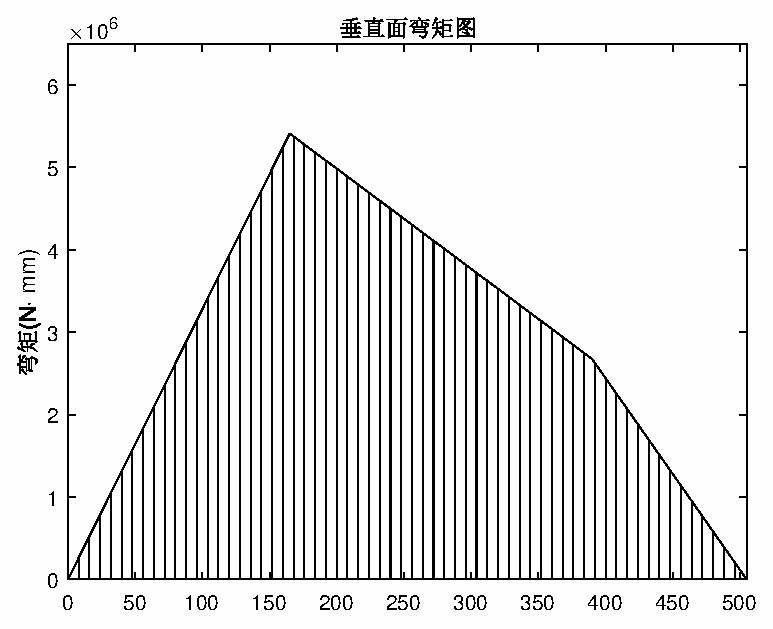
\includegraphics[width=0.6\textwidth]{./pic/wan_v.eps}\\
		\caption{垂直面弯矩图}\label{wan-v}
	\end{figure}

	计算水平面弯矩图,如图\ref{wan-h}所示。主要计算如下:

	截面b:
		\begin{align}
			M_{bh}' &= 165F_{2h} = 165\times 7133 = 1176945\\
			M_{bh}'' &= M_{bh}'+ \dfrac{F_{3a}d_3}{2} = 1176945+ \dfrac{8316\times 170}{2} = 1883805
		\end{align}
		
	截面c:
		\begin{align}
			M_{ch}' &= 115F_{1h} = 115\times 5357 = 616055\\
			M_{ch}'' &= M_{ch}' - \dfrac{F_{2a}d_2}{2} = 616055 - \dfrac{2530\times 688}{2} = -254265
		\end{align}

	\begin{figure}[H]
		\centering
		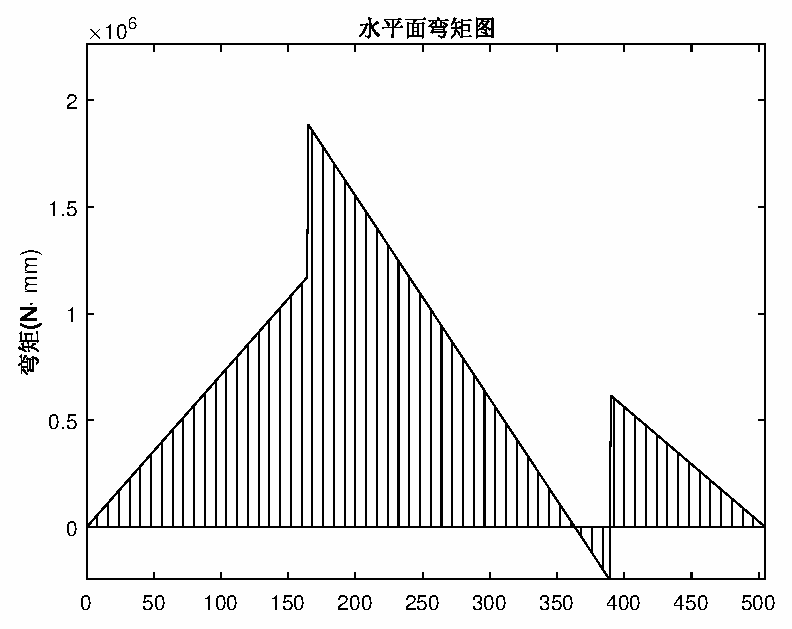
\includegraphics[width=0.6\textwidth]{./pic/wan_h.eps}\\
		\caption{水平面弯矩图}\label{wan-h}
	\end{figure}

	计算合成弯矩图,如图\ref{wan-he}所示。主要计算如下:
	
		截面b:
			\begin{align}
				M^{′}_{b}=\sqrt{M^{′2}_{bH}+M^{2}_{bV}}=\sqrt{1176945^2 + 5409690^2}=5536239(N\cdot mm)\\
				M^{″}_{b}=\sqrt{M^{″2}_{bH}+M^{2}_{bV}}=\sqrt{1883805^2 + 5409690^2}=5728304(N\cdot mm)
			\end{align}
			
		截面c:
			\begin{align}
				M^{′}_{c}=\sqrt{M^{′2}_{cH}+M^{2}_{cV}}=\sqrt{616055^2 + 2674900^2}=2744925(N\cdot mm)\\
				M^{″}_{c}=\sqrt{M^{″2}_{cH}+M^{2}_{cV}}=\sqrt{254265^2 + 2674900^2}=2686958(N\cdot mm)
			\end{align}

	\begin{figure}[H]
		\centering
		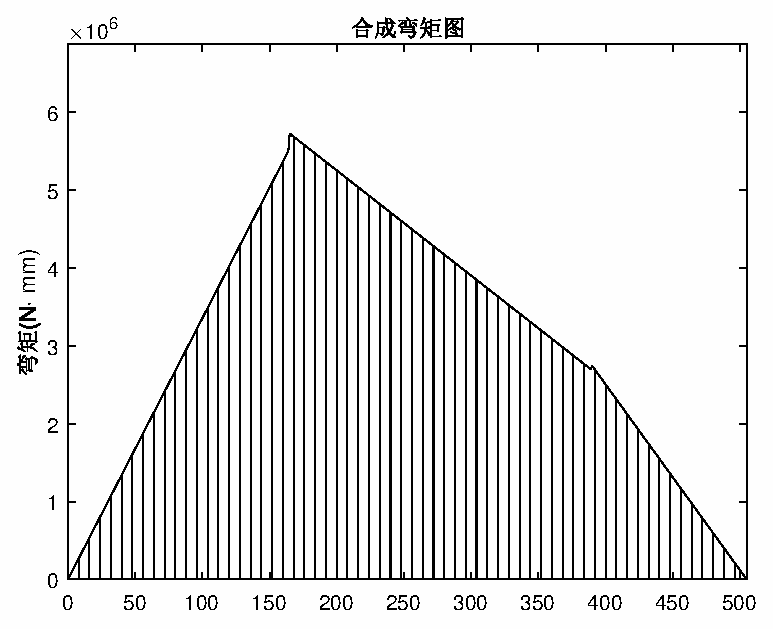
\includegraphics[width=0.6\textwidth]{./pic/wan_he.eps}\\
		\caption{合成弯矩图}\label{wan-he}
	\end{figure}

	\subsection{绘制扭矩图}
	由所给条件可知,$T=3.82\times 10^6 (N\cdot mm)$,采用的材料为正火处理的45号钢,其$\sigma_B =600 MPa$,查得数据\footnote{陈秀宁,顾大强.机械设计.浙江大学出版社,2010,表(12-3)}$[\sigma_{-1}]_b = 55 Mpa$,$[\sigma_{0}]_b =95MPa$,故$\alpha = \dfrac{55}{95} \approx 0.58$,
	\[\alpha T=0.58\times 3.82\times 10^6 =2.2156\times 10^6 (N\cdot mm)\]

	\begin{figure}[H]
		\centering
		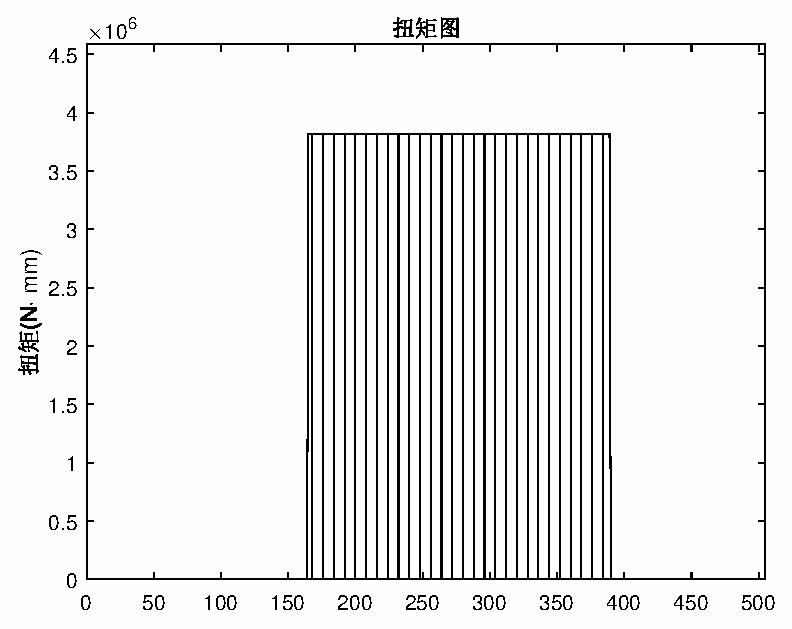
\includegraphics[width=0.6\textwidth]{./pic/niu.eps}\\
		\caption{扭矩图}\label{niu}
	\end{figure}

	\subsection{绘制当量弯矩图}
	计算当量弯矩图,计算结果如图\ref{wan-d}所示。主要计算如下:
	
		截面b:
			\begin{align}
				M^{′}_{be} &=5536239(N\cdot mm)\\
				M^{″}_{be} &=\sqrt{M^{″2}_{b}+(\alpha T)^2}=\sqrt{5728304^2 +(2.2156\times 10^6)^2}=6141852(N\cdot mm)
			\end{align}
			
		截面c:
			\begin{align}
				M^{′}_{ce} &=2744925(N\cdot mm)\\
				M^{″}_{ce} &=\sqrt{M^{″2}_{c}+(\alpha T)^2}=\sqrt{2686958^2 +(2.2156\times 10^6)^2}=3482618(N\cdot mm)
			\end{align}

	\begin{figure}[H]
		\centering
		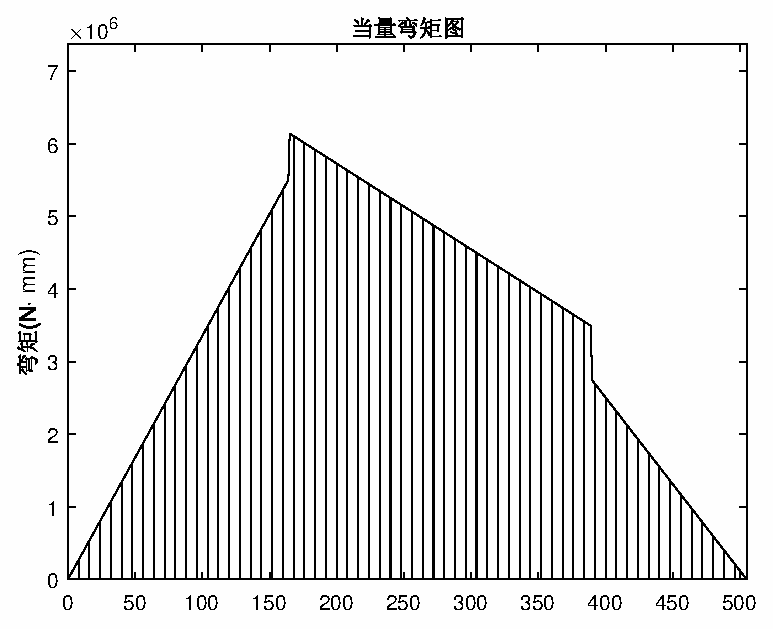
\includegraphics[width=0.6\textwidth]{./pic/wan_d.eps}\\
		\caption{当量弯矩图}\label{wan-d}
	\end{figure}

	\subsection{分别计算截面的直径}
	根据当量弯矩计算截面b和c处的直径,\footnote{陈秀宁,顾大强.机械设计.浙江大学出版社,2010,式(12-4)}
	\begin{align}
		d_b &\geq \sqrt[3]{\frac{M^{″}_{be}}{0.1[\sigma_{-1}]_b}}=\sqrt[3]{\frac{6141852}{0.1\times 60}}=100.78(mm)\\
		d_c &\geq \sqrt[3]{\frac{M^{″}_{ce}}{0.1[\sigma_{-1}]_b}}=\sqrt[3]{\frac{3482618}{0.1\times 60}}=83.42(mm)
	\end{align}
	初步设计时这两个地方的直径均设置为110mm,因此满足条件。

\section{强度校核}
	对截面b进行疲劳强度校核,查表\footnote{陈秀宁,顾大强.机械设计.浙江大学出版社,2010,表(12-1)}可得,$\sigma_{-1}=240MPa$,$\tau_{-1}=140MPa$。其弯曲应力为
	\begin{align}
		\sigma_a &=\frac{M^{″}_{b}}{W}=\frac{32M^{′}_{b}}{\pi d^3}=\frac{32\times 5728304}{3.14\times 108^3}=46.34(MPa)\\
		\sigma_m &=0
	\end{align}

	其扭转应力为
	\begin{align}
		\tau_a &=\frac{1}{2}\tau =\frac{T}{2W_T}=\frac{8T}{\pi d^3}=\frac{8\times 3.82\times 10^6}{3.14\times 108^3}=7.73(Mpa)\\
		\tau_m &=\frac{1}{2}\tau =7.73(MPa)
	\end{align}

	所选用的材料为45号钢,则其弯曲等效系数$\psi_{\sigma}=0.1\sim 0.2$,此处取0.2,轴的剪切等效系数,$\psi_{\tau} = 0.5\psi_{\sigma} = 0.1$。
	
	查表\footnote{陈秀宁,顾大强.机械设计.浙江大学出版社,2010,表(12-4)},此处采用的是A型键槽,则得键槽处的弯曲、扭转有效应力集中系数为,$k_{\sigma}=1.76$,$k_{\tau}=1.54$。

	查表\footnote{陈秀宁,顾大强.机械设计.浙江大学出版社,2010,表(12-7)}得到,轴的直径在100-120之间,则弯曲、扭剪时轴的绝对尺寸系数为,$\varepsilon_{\sigma}=0.70$,$\varepsilon_{\tau}=0.70$。

	查表\footnote{陈秀宁,顾大强.机械设计.浙江大学出版社,2010,表(12-8)}得到,选择轴的表面质量系数$\beta = 0.90$。

	按无限寿命考虑,取寿命系数$K_N =1$,此时材质均匀,载荷与应力计算精确,故取$[s]=1.5$,带入式子计算
	\begin{align}
		S_{\sigma} &=\dfrac{K_N \sigma_{-1}}{\dfrac{k_{\sigma}}{\varepsilon_{\sigma}\beta}\sigma_{\alpha}+\psi_{\sigma}\sigma_m}=\dfrac{1\times 240\times 0.70\times 0.90}{1.82\times 46.34}=1.79\\
		S_{\tau} &=\dfrac{K_N \tau_{-1}}{\dfrac{k_{\tau}}{\varepsilon_{\tau}\beta}\tau_{\alpha}+\psi_{\tau}\tau_m}=\dfrac{1\times 140}{\dfrac{1.62}{0.70\times 0.90}\times 7.73+0.1\times 7.73}=6.78\\
		S &=\frac{S_{\sigma}S_{\tau}}{\sqrt{S^2_{\sigma}+S^2_{\tau}}}=\frac{2.05\times 7.51}{\sqrt{2.05^2+7.51^2}}=1.73>[S]
	\end{align}
	因此,轴的b 截面具有足够的疲劳强度、安全。

	b截面与c截面相同,但c截面的合成弯矩比b截面小,同时两个截面所受的扭矩相同,所以c截面也有足够的疲劳强度、安全。

\section{其他零件}

\subsection{轴承选择}\label{zhoucheng}
	根据估算的直径,轮毂宽度,分别在轴的两端安装一对7218C\footnote{GB/T 292-1994}角接触轴承,轴承宽度为30mm,两端的轴承均使用套筒定位。
	\minpic{zhoucheng.png}{角接触轴承示意图}

	\begin{table}[H]
		\centering
		\begin{tabular}{cccc}
			\toprule 
			$d,D,B$ & $C_r,C_0$ & $d_2,D_2,a,r,r_1$ & $d_a,D_a,r_a$\\
			\midrule 
			90,160,30 & 122,105 & 111.7,138.4,31.7,2,2 & 100,150,2\\
			\bottomrule
		\end{tabular}
		\caption{角接触轴承参数}
		\label{tab:arg}
	\end{table}

\subsection{套筒}
	取套筒外径为110mm,内径与轴承内径相同,取90mm,套筒与齿轮配合处应高于齿轮,取齿轮孔径为110mm,套筒与齿轮接触处增加其外径,方便与齿轮配合。套筒尺寸如图所示。
	\midpic{taotong.png}{套筒结构示意图}

\subsection{键}
	轴与两齿轮直接均采用平键连接,键槽的尺寸根据轴的直径确定,查机械设计手册\footnote{GB/T 1095/2003},键的尺寸为$b\times h = 32\times 18$,键槽的宽度基本尺寸为32,采用正常连接,轴N9.0~-0.062,毂JS9,$\pm 0.031$,深度尺寸,轴11.0+0.20,毂7.4+0.20,半径r取0.5。
	\midpic{jian.png}{键的剖面尺寸示意图}
	键的长度根据式子\ref{jianchang}确定。
	\begin{equation}\label{jianchang}
		L_c \geq \frac{4T}{dh[\sigma_p]}
	\end{equation}
	带入数据计算得到
	\[L_c \geq 88mm\]
	取输入齿轮处的平键长度为100mm,输出齿轮处的平键长度为150mm。
\subsection{轴承寿命}
	所选轴承为单列角接触轴承,型号为7218C,$C_0 = 105$。
	\subsubsection{计算轴承受力}
	轴承所受总径向力为
	\begin{align}
		F_1 & = \sqrt{F_{h1}^2+F_{v1}^2} = 23543N\\
		F_2 & = \sqrt{F_{h2}^2+F_{v2}^2} = 33878N
	\end{align}
	主轴受到的轴向力为
	\begin{equation}
		F_a = F_{a3} - F_{a2} = 5786N
	\end{equation}
	计算可得
	\begin{equation}
		\frac{F_a}{C_0} = 0.0551
	\end{equation}
	查表得$e = 0.43$\footnote{陈秀宁,顾大强.机械设计.浙江大学出版社,2010,表(14-10)},左右两轴承的附加轴向力为
	\begin{equation}
		S_1 = 10124N,S_2 = 14508N
	\end{equation}。
	由于$S_1 - F_a \leq S_2$,所以右边轴承被压紧,左边轴承被放松,由此可得:
	\begin{align}
		F_{a1} & = S_2+F_a = 20354N\\
		F_{a2} & = S_2 = 14568N
	\end{align}
	\subsubsection{计算当量载荷}
	对于轴承1,取$K_p = 1$,
	\begin{equation}
		\dfrac{F_{a1}}{C_0} = 0.1938
	\end{equation}
	查表取值得:$e_1 = 0.51$\footnote{陈秀宁,顾大强.机械设计.浙江大学出版社,2010,表(14-10)},计算\begin{equation}
		\dfrac{F_{a1}}{F_1} = \dfrac{20354}{23543} = 0.86 > 0.51
	\end{equation}
	查表取值得:$X_1 = 0.44,Y_1 = 1.09$,则
	\[P_1 = K_p(X_1F_1 + Y_1F_{a1} = 32545N\]

	对于轴承2,取$K_p = 1$,
	\begin{equation}
		\dfrac{F_{a2}}{C_0} = 0.1387
	\end{equation}
	查表取值得:$e_1 = 0.51$\footnote{陈秀宁,顾大强.机械设计.浙江大学出版社,2010,表(14-10)},计算\begin{equation}
		\dfrac{F_{a2}}{F_2} = \dfrac{14568}{33878} = 0.43 < 0.48
	\end{equation}
	查表取值得:$X_1 = 1,Y_1 =0$,则
	\[P_1 = K_p(X_1F_1 + Y_1F_{a1} = 33878N \]

	\subsubsection{计算$L_h$}
	因为$P_1 < P_2$,故按轴承2计算轴承寿命
	\begin{equation}
		L_{10h}=\frac{10^6}{60n}(\frac{C}{P})^{\varepsilon}=\frac{10^6}{60\times 100}(\frac{198000}{55046})^3 = 7783h
	\end{equation}
	即轴承寿命为7783h。

\section{装配结构草图}
	见附件。
